\documentclass[8pt]{beamer}\usepackage[]{graphicx}\usepackage[]{color}


\usetheme{metropolis}           % Use metropolis theme
\usepackage{amsmath}
\usepackage{mathrsfs}
\usepackage{tabularx}
\usepackage{tikz}
\usetikzlibrary{patterns}

% For custom oversets
\usepackage{accents}

% For addmargin
\usepackage{scrextend}


\usepackage[style=authoryear]{biblatex}
\addbibresource{references.bib}
\usepackage{cleveref}
\renewcommand*{\bibfont}{\footnotesize}


\def\coingrid{
\draw[step=1cm,gray,very thin] (0,0) grid (2,3);
\node[left, color=blue] at (0, 2.5) {Coin TT};
\node[left, color=blue] at (0, 1.5) {Coin HT};
\node[left, color=blue] at (0, 0.5) {Coin HH};
\node[above, color=purple] at (0.5, 3) {Side 1};
\node[above, color=purple] at (1.5, 3) {Side 2};
\node[below right, color=black] at (0, 3) {\tiny TT1};
\node[below right, color=black] at (0, 2) {\tiny HT1};
\node[below right, color=black] at (0, 1) {\tiny HH1};
\node[below right, color=black] at (1, 3) {\tiny TT2};
\node[below right, color=black] at (1, 2) {\tiny HT2};
\node[below right, color=black] at (1, 1) {\tiny HH2};
}

\def\rectfill#1#2#3#4{
\draw[pattern=#1, pattern color=#2] (#3,#4) rectangle (#3 + 1,#4 + 1);
}


\def\truth{${\color{red}\times}$}

\def\heads{

\begin{tikzpicture}[scale=0.30]
    \rectfill{north west lines}{blue}{0}{1}
\end{tikzpicture}
}

\def\ttcoin{

\begin{tikzpicture}[scale=0.30]
    \draw[draw=lime, thick] (0, 1) rectangle ++(1, 1);
\end{tikzpicture}
}

\def\htcoin{

\begin{tikzpicture}[scale=0.30]
    \draw[draw=red, thick] (0, 1) rectangle ++(1, 1);
\end{tikzpicture}
}

\def\hhcoin{

\begin{tikzpicture}[scale=0.30]
    \draw[draw=cyan, thick] (0, 1) rectangle ++(1, 1);
\end{tikzpicture}
}


\def\hiprop{

\begin{tikzpicture}[scale=0.30]
    \rectfill{north east lines}{red}{0}{1}
\end{tikzpicture}
}



\def\setminipage{

\begin{minipage}{0.38\textwidth}
    \begin{center}
    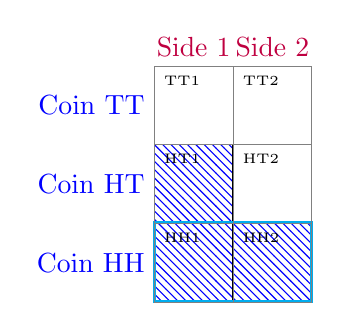
\begin{tikzpicture}
        \rectfill{north west lines}{blue}{0}{0}
        \rectfill{north west lines}{blue}{0}{1}
        \rectfill{north west lines}{blue}{1}{0}
        % \draw[draw=red, very thick] (0, 1) rectangle ++(2, 1);
        % \draw[draw=lime, very thick] (0, 2.01) rectangle ++(2, 1);
        \draw[draw=cyan, very thick] (0, 0.01) rectangle ++(2, 1);
        \coingrid{}
    \end{tikzpicture}
\end{center}
\end{minipage}
\begin{minipage}{0.58\textwidth}
    %
    \heads{} We observe heads = $HT1 \lor HH1 \lor HH2$

    % \ttcoin{} We chose the TT coin = $TT1 \lor TT2$

    % \htcoin{} We chose the HT coin = $HT1 \lor HT2$

    \hhcoin{} We chose the HH coin = $HH1 \lor HH2$

    Recall that the truth \truth{} lies in exactly one cell.

\end{minipage}

}


\def\pmminipage{

\begin{minipage}{0.38\textwidth}
    \begin{center}
    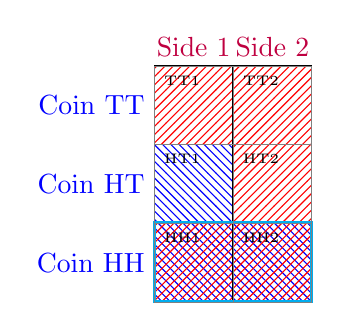
\begin{tikzpicture}
        \rectfill{north west lines}{blue}{0}{0}
        \rectfill{north west lines}{blue}{0}{1}
        \rectfill{north west lines}{blue}{1}{0}
        \rectfill{north east lines}{red}{0}{0}
        \rectfill{north east lines}{red}{1}{0}
        \rectfill{north east lines}{red}{1}{1}
        \rectfill{north east lines}{red}{1}{2}
        \rectfill{north east lines}{red}{0}{2}

        \draw[draw=cyan, very thick] (0, 0.01) rectangle ++(2, 1);
        \coingrid{}
    \end{tikzpicture}
\end{center}
\end{minipage}
\begin{minipage}{0.58\textwidth}
    %
    \heads{} $e$ = We observe heads\\
    \hhcoin{} $h$  = We chose the HH coin\\
    \heads{} $h_D$ = Inductive component = $h \lor e = e$\\
    \hiprop{} $h_I$ = Inductive component = $h \lor \lnot e$

    \vspace{1em}
    We can write $h = h_D \land h_I$.\\

    Note also that $h \subseteq e$ so $h_D = e$.
    %
\end{minipage}

}


\def\p#1{\mathbb{P}\left(#1\right)}
\def\q#1{\mathbb{Q}\left(#1\right)}
\def\y{y}
\def\z{z}
\def\normz{\mathcal{N}(z)}
\def\etahat{\hat{\eta}}
\def\ellhat{\hat{\ell}}
\def\sumn{\sum_{n=1}^N}
\def\meann{\frac{1}{N} \sumn}
\newcommand{\etastar}{\accentset{*}{\eta}}
\def\Z{\mathcal{Z}}
\def\expect#1#2{\mathbb{E}_{#1}\left[#2\right]}
\def\kl#1{\mathrm{KL}\left(#1\right)}
\def\klhat#1{\widehat{\mathrm{KL}}\left(#1\right)}
\def\ind#1{1\left(#1\right)}

\DeclareMathOperator*{\argmax}{\mathrm{argmax}}
\DeclareMathOperator*{\argmin}{\mathrm{argmin}}
\DeclareMathOperator*{\esssup}{\mathrm{esssup}}
\DeclareMathOperator*{\essinf}{\mathrm{essinf}}
\DeclareMathOperator*{\argsup}{\mathrm{argsup}}
\DeclareMathOperator*{\arginf}{\mathrm{arginf}}

\title{Inductive logic: Introduction and context}
\author{Ryan Giordano}
\date{Sep 23rd, 2022}
\institute{Massachusetts Institute of Technology}

\begin{document}




%%%%%%%%%%%%%%%%%%%%%%%%%%%%%%%%%%%%%%%%%%%%%%%%%%%%%%%%%%%%%%%%%%%%%%%
%%%%%%%%%%%%%%%%%%%%%%%%%%%%%%%%%%%%%%%%%%%%%%%%%%%%%%%%%%%%%%%%%%%%%%%
%%%%%%%%%%%%%%%%%%%%%%%%%%%%%%%%%%%%%%%%%%%%%%%%%%%%%%%%%%%%%%%%%%%%%%%

\begin{frame}{Outline}
%
\begin{itemize}
%
\item Logic
\item Deduction and induction
\item Classes of inductive questions (from philosophical induction to probability)
\item Extreme resolutions: ``Bayesian,'' ``falsificationist,'' ``conventionalist''
%
\end{itemize}
%
\end{frame}

%%%%%%%%%%%%%%%%%%%%%%%%%%%%%%%%%%%%%%%%%%%%%%%%%%%%%%%%%%%%%%%%%%%%%%%
%%%%%%%%%%%%%%%%%%%%%%%%%%%%%%%%%%%%%%%%%%%%%%%%%%%%%%%%%%%%%%%%%%%%%%%
%%%%%%%%%%%%%%%%%%%%%%%%%%%%%%%%%%%%%%%%%%%%%%%%%%%%%%%%%%%%%%%%%%%%%%%

\begin{frame}{Logic}
%
As far as we know, among the great ancient civilizations, only the Greeks
studied the formal validity of argumentation, a.k.a., logic
(\cite{shenefelt:2013:ifathenb}).  This presentation will borrow a lot from the
lucid and readable reference \cite{hacking:2001:introduction}.

\pause
Logic studies the {\em validity} of an argument, not the {\em truth} of
its conclusions.

An argument is valid if it is logically sound.

A proposition is a statement which is either true or false.

\vspace{1em}
\textbf{Example: }\\
If James wants a job, then he will get a haircut tomorrow.\\
James will get a haircut tomorrow.\\
So: James wants a job.

\vspace{1em}
If James wants a job, then he will get a haircut tomorrow.\\
James wants a job.\\
So: James will get a haircut tomorrow.

\pause
\vspace{1em}
\textbf{Questions:} \\
Which argument is valid?  \\
What are the propositions?\\
Which propositions are true?
%
\end{frame}



%%%%%%%%%%%%%%%%%%%%%%%%%%%%%%%%%%%%%%%%%%%%%%%%%%%%%%%%%%%%%%%%%%%%%%%
%%%%%%%%%%%%%%%%%%%%%%%%%%%%%%%%%%%%%%%%%%%%%%%%%%%%%%%%%%%%%%%%%%%%%%%
%%%%%%%%%%%%%%%%%%%%%%%%%%%%%%%%%%%%%%%%%%%%%%%%%%%%%%%%%%%%%%%%%%%%%%%

\begin{frame}{Logic}
%
\textbf{Which of these arguments are valid?}
(\cite[Ch.1 Question 7]{hacking:2001:introduction})

%
\begin{itemize}
%
\item I follow three major league teams.  Most of their top hitters chew
tobacco at the plate.\\
$\Rightarrow$ Chewing tobacco improves batting average.
%
\item The top six hitters in the National League chew tobacco at the plate.\\
$\Rightarrow$ Chewing tobacco improves batting average.
%
\item A study by the American Dental Association of 158 players on
seven major league teams during the 1988 season showed that the mean batting
average for chewers was 0.238 compared to 0.248 for non-users.  Abstainers
also had a higher fielding average.\\
$\Rightarrow$ Chewing tobacco does not improve batting average.
%
\item In 1921, every major league pitcher who chewed tobacco when up to
bat had a higher batting average than any major league pitcher who did
not.\\
$\Rightarrow$ Chewing tobacco does not improve batting average.
%
\end{itemize}
%
\pause
\textbf{None of them are valid.}

But some are better than others.
In what sense?  In any logical sense?
%
\end{frame}


%%%%%%%%%%%%%%%%%%%%%%%%%%%%%%%%%%%%%%%%%%%%%%%%%%%%%%%%%%%%%%%%%%%%%%%
%%%%%%%%%%%%%%%%%%%%%%%%%%%%%%%%%%%%%%%%%%%%%%%%%%%%%%%%%%%%%%%%%%%%%%%
%%%%%%%%%%%%%%%%%%%%%%%%%%%%%%%%%%%%%%%%%%%%%%%%%%%%%%%%%%%%%%%%%%%%%%%

\begin{frame}{Logic}

% Aristotle identified four ``categorical propositions'' that form the basis
% of his logic:
%
% %
% \begin{itemize}
% %
% \item All As are Bs.
% \item No As are Bs.
% \item Some As are Bs.
% \item Some As are not Bs.
% %
% \end{itemize}
% %
The Stoics identify the following syllogisms, purported patterns of
valid inference:
%
\begin{itemize}
%
\item \emph{Modus Ponens}: If A, then B.  A.  Therefore, B.
\item \emph{Modus Tollens}: If A, then B.  Not B.  Therefore, not A.
\item The Hypothetical Syllogism: If A, then B.  If B, then C.  Therefore, if A, then C.
\item The Conjunctive Syllogism: Not both A and B.  A.  Therefore, not B.
\item The Dilemma: If A, then B.  If C, then B.  A or C.  Therefore, B.
\item The Disjunctive Syllogism: A or B.  But not A.  Therefore, B.
%
\end{itemize}
%
\textbf{Proposition:} If we begin with true propositions, and combine
them according to the above syllogisms, we necessarily reach a true conclusion.

Reasoning in this way is called \textbf{deductive reasoning}.


% Humans are free to construct ``logics,'' which may
% or may not actually produce something we are willing to call truth.  To
% paraphrase \cite{hacking:2016:logic}:
%
% \begin{block}{}
% %
% ``The problem of the [logic] is to state a set of principles
% which entail the validity of all correct [inference], and which do not
% imply that any fallacious inference is valid.''
% %
% \end{block}
%
\end{frame}


%%%%%%%%%%%%%%%%%%%%%%%%%%%%%%%%%%%%%%%%%%%%%%%%%%%%%%%%%%%%%%%%%%%%%%%
%%%%%%%%%%%%%%%%%%%%%%%%%%%%%%%%%%%%%%%%%%%%%%%%%%%%%%%%%%%%%%%%%%%%%%%
%%%%%%%%%%%%%%%%%%%%%%%%%%%%%%%%%%%%%%%%%%%%%%%%%%%%%%%%%%%%%%%%%%%%%%%


\begin{frame}{Example}
%
Set theory can provide a means to visualize and analyze logical reasoning.
Here is an example that I think may be useful.\footnote{I cooked this up and
have no idea how standard this is.  I realized preparing for this how
little I know about logic.}


Suppose a bag contains three coins: one regular coin (HT), one with both
faces tails (TT), and one with both faces heads (HH).  The coin is flipped,
and either the first or second side comes up.

Exactly one possible outcome
of coin $\times$ side occurs; call this the ``truth.''

\begin{minipage}{0.38\textwidth}
    \begin{center}
    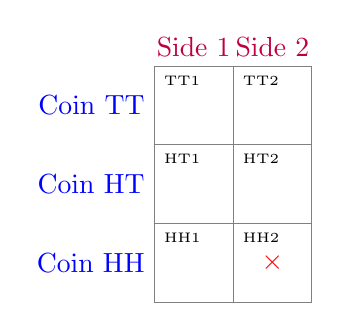
\begin{tikzpicture}
        \coingrid{}
        \node[color=red] at (1.5, 0.5) {$\times$};
    \end{tikzpicture}
\end{center}
\end{minipage}
\begin{minipage}{0.58\textwidth}
    %
    \textbf{Example:}\\
    Coin HH was picked and the second side came up (HH2).

    \vspace{1em} In this context, classical propositional logic can be
    represented as set operations.
    %
\end{minipage}
%
\end{frame}

%%%%%%%%%%%%%%%%%%%%%%%%%%%%%%%%%%%%%%%%%%%%%%%%%%%%%%%%%%%%%%%%%%%%%%%
%%%%%%%%%%%%%%%%%%%%%%%%%%%%%%%%%%%%%%%%%%%%%%%%%%%%%%%%%%%%%%%%%%%%%%%
%%%%%%%%%%%%%%%%%%%%%%%%%%%%%%%%%%%%%%%%%%%%%%%%%%%%%%%%%%%%%%%%%%%%%%%

\begin{frame}{Example}

\setminipage{}
\pause
\textbf{Questions:}

Suppose we observe heads (so we know \truth{} $\in$ \heads{}).

What can we deduce about whether we drew the TT coin?

What can we deduce about whether we drew the HT coin?

What can we deduce about whether we drew the HH coin?

\textbf{Hint:}
%
Note that \heads{} $\subseteq$ \ttcoin{}$^c$.


\end{frame}


%%%%%%%%%%%%%%%%%%%%%%%%%%%%%%%%%%%%%%%%%%%%%%%%%%%%%%%%%%%%%%%%%%%%%%%
%%%%%%%%%%%%%%%%%%%%%%%%%%%%%%%%%%%%%%%%%%%%%%%%%%%%%%%%%%%%%%%%%%%%%%%
%%%%%%%%%%%%%%%%%%%%%%%%%%%%%%%%%%%%%%%%%%%%%%%%%%%%%%%%%%%%%%%%%%%%%%%

\begin{frame}{Example}
    \setminipage{}

\textbf{In general:} Set inclusion is the same as deductive entailment:

$A$ is true and $A \subseteq B$ implies that $B$ is true.
This is the set version of {\em modus ponens}.

(\textbf{Optional exercise:} Rewrite the other logical syllogisms as set operations.)

If $A$ is true, and $A$ overlaps partially with $B$, nothing about $B$
follows deductively, because \textbf{you might be wrong}.

\end{frame}

%%%%%%%%%%%%%%%%%%%%%%%%%%%%%%%%%%%%%%%%%%%%%%%%%%%%%%%%%%%%%%%%%%%%%%%
%%%%%%%%%%%%%%%%%%%%%%%%%%%%%%%%%%%%%%%%%%%%%%%%%%%%%%%%%%%%%%%%%%%%%%%
%%%%%%%%%%%%%%%%%%%%%%%%%%%%%%%%%%%%%%%%%%%%%%%%%%%%%%%%%%%%%%%%%%%%%%%

\begin{frame}{Example}
    \setminipage{}

And yet it seems silly to claim that observing a heads tells you
nothing about whether you have chosen the HH coin.

After all,  the ``prior'' $p(\textrm{HH coin}) = 1/3$,
but the ``posterior'' $p(\textrm{HH coin} | \textrm{heads}) =
2/3$.

\pause

\textbf{Reasoning that goes beyond deduction is called ``induction.''} (It is
also sometimes called ``ampliative'' reasoning because it concludes more than is
given by the premises.)

\pause
\textbf{Questions:}\\
Is induction even possible?  If so, how?\\
% Can the probability calculus provide the key to a valid inductive logic?\\
\textbf{As we will see, early statisticians were extremely preoccupied
with this question.}\footnote{Or I think we will see this,
I haven't read most of these papers yet either.}


\end{frame}



%%%%%%%%%%%%%%%%%%%%%%%%%%%%%%%%%%%%%%%%%%%%%%%%%%%%%%%%%%%%%%%%%%%%%%%
%%%%%%%%%%%%%%%%%%%%%%%%%%%%%%%%%%%%%%%%%%%%%%%%%%%%%%%%%%%%%%%%%%%%%%%
%%%%%%%%%%%%%%%%%%%%%%%%%%%%%%%%%%%%%%%%%%%%%%%%%%%%%%%%%%%%%%%%%%%%%%%

\begin{frame}{The European Enlightenment was an exciting time}

%\vspace{3em}
%
\begin{minipage}{0.6 \textwidth}
%
{\footnotesize
\begin{itemize}
%
\item 1657: Huygens' The Value of all Chances in Games of Fortune
\item 1687: Newton's {\em Prinicipia Mathematica}
\item 1690: Locke's Essay Concerning Human Understanding
\item 1713 Bernoulli's The Art of Conjecturing
\item 1718 De Moivre's The Doctrine of Chances
\item 1739: \textbf{Hume's An Enquiry Concerning Human Understanding}
\item 1751-1772: Diderot's Encyclopedia
\item 1763: Bayes' An Essay towards solving a Problem in the Doctrine of Chances
\item 1770: Euler's Foundations of integral calculus
\item 1776: The American Revolution
\item 1776: Adam Smith's The Wealth of Nations
\item 1789: The French Revolution
\item 1812: Laplace's Analytic Theory of Probabilities
\vspace{1em}
%
\end{itemize}
}
%
\end{minipage}
\begin{minipage}{0.35 \textwidth}
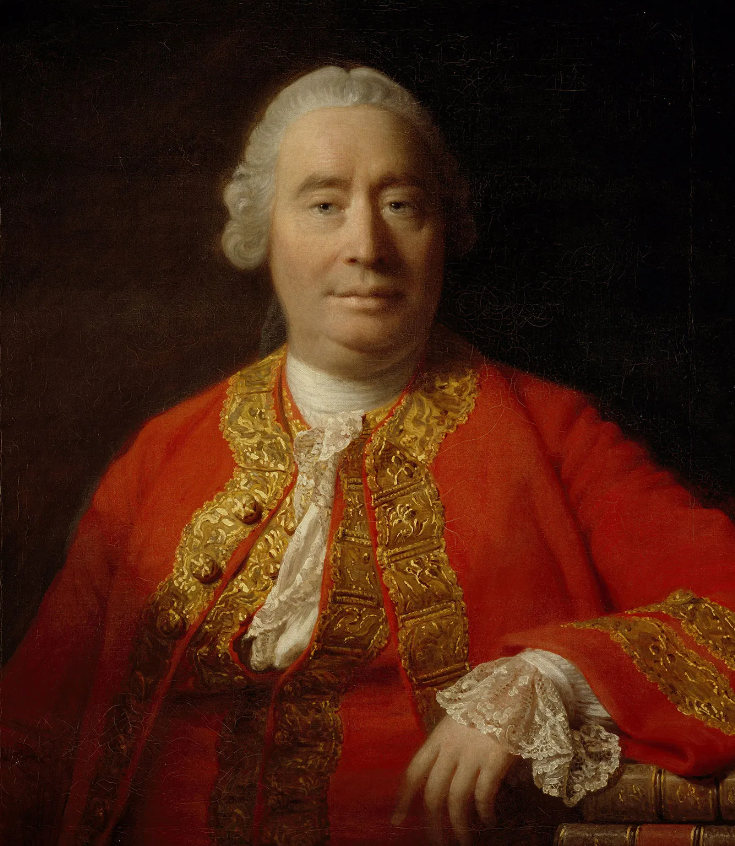
\includegraphics[width=0.9 \textwidth]{Hume.png}
\end{minipage}
%
%\vspace{3em}
\pause
\textbf{Foundations, rigor, and revolution} were all in the air.

\pause
\textbf{Is induction even possible?  If so, how?}

We have asked this question in the setting when it has, arguably, the best
chance of being possible (a well-defined probability setup).

Hume asked it in much, much greater generality.

\end{frame}

%%%%%%%%%%%%%%%%%%%%%%%%%%%%%%%%%%%%%%%%%%%%%%%%%%%%%%%%%%%%%%%%%%%%%%%
%%%%%%%%%%%%%%%%%%%%%%%%%%%%%%%%%%%%%%%%%%%%%%%%%%%%%%%%%%%%%%%%%%%%%%%
%%%%%%%%%%%%%%%%%%%%%%%%%%%%%%%%%%%%%%%%%%%%%%%%%%%%%%%%%%%%%%%%%%%%%%%

\begin{frame}{Hume}

\textbf{Is induction even possible?  If so, how?}
%
\begin{enumerate}
%
\item All questions are ``Relations of Ideas'' or ``Matters of Fact.''
\item ``Relations of Ideas'' are deductive, certain, mathematical.
\item ``Matters of Fact'' are sensory, experiental, contingent, local
in time and space.
\item The content of ideas is entirely matters of fact.
%
\end{enumerate}
%
Here, ``matters of fact'' correspond to propositions, and
``relations of ideas'' to deductive logic.

\textbf{Hume's question:} We believe much more about the world than we
experience directly.  What is the foundation of this belief?  Is it
experience?  Is it deduction?  What combination of the two?

\end{frame}


%%%%%%%%%%%%%%%%%%%%%%%%%%%%%%%%%%%%%%%%%%%%%%%%%%%%%%%%%%%%%%%%%%%%%%%
%%%%%%%%%%%%%%%%%%%%%%%%%%%%%%%%%%%%%%%%%%%%%%%%%%%%%%%%%%%%%%%%%%%%%%%
%%%%%%%%%%%%%%%%%%%%%%%%%%%%%%%%%%%%%%%%%%%%%%%%%%%%%%%%%%%%%%%%%%%%%%%

\begin{frame}{Cause and Effect}

Hume specifies three ways ideas can be associated:
%
\begin{enumerate}
%
\item Resemblance
\item Co-occurence
\item Cause and effect
%
\end{enumerate}
%
Hume argues that it is because of cause and effect that we extrapolate
from local, transient experiences.

\pause
\textbf{Question:} What is the difference between Hume's co-occurence and
cause and effect?

\pause
\textbf{Question:} What is the difference between Hume's
cause and effect and Judea Pearl's?

\pause
\textbf{Question:} What is the difference between Hume's
cause and effect and the counterfactulas of the Neyman-Rubin framework?

\end{frame}

%%%%%%%%%%%%%%%%%%%%%%%%%%%%%%%%%%%%%%%%%%%%%%%%%%%%%%%%%%%%%%%%%%%%%%%
%%%%%%%%%%%%%%%%%%%%%%%%%%%%%%%%%%%%%%%%%%%%%%%%%%%%%%%%%%%%%%%%%%%%%%%
%%%%%%%%%%%%%%%%%%%%%%%%%%%%%%%%%%%%%%%%%%%%%%%%%%%%%%%%%%%%%%%%%%%%%%%

\begin{frame}{Cause and Effect}

Cause and effect differs from co-occurence by being \textbf{necessary}.

So how do we establish that something is necessary?  Can we establish
it by deduction?  By experience?

\pause
\textbf{Not by deduction:}

\begin{addmargin}[2em]{2em}% 1em left, 2em right
``I say then that, even after we have experience of the operations of
cause and effect, our conclusions from that experience are not founded
on reasoning, or on any process of the understanding.''  (28)
\end{addmargin}

\pause
\textbf{And not by experience:}
\begin{addmargin}[2em]{2em}% 1em left, 2em right
``For all inferences from experience suppose, as their foundation, that
the future will resemble the past, and that similar powers will be conjoined
with similar sensible qualities.  If there be any suspicion that the course
of nature may change, and that the past may be no rule for the future,
all experience becomes useless, and can give rise to no inference
or conclusion.'' (32)
\end{addmargin}

\pause
Hume's answer: ``Custom.''

\pause

\textbf{Question:}  What is Hume saying about inductive reasoning?

\textbf{Question:}  In Hume's view, what classes of questions fall
under the category of inductive reasoning?

\end{frame}


%%%%%%%%%%%%%%%%%%%%%%%%%%%%%%%%%%%%%%%%%%%%%%%%%%%%%%%%%%%%%%%%%%%%%%%
%%%%%%%%%%%%%%%%%%%%%%%%%%%%%%%%%%%%%%%%%%%%%%%%%%%%%%%%%%%%%%%%%%%%%%%
%%%%%%%%%%%%%%%%%%%%%%%%%%%%%%%%%%%%%%%%%%%%%%%%%%%%%%%%%%%%%%%%%%%%%%%


\begin{frame}{Hume on science}

Hume writes:

\begin{addmargin}[2em]{2em}% 1em left, 2em right
    ``Elasticity, gravity, cohesion of parts, communication of motion
    by impulse; these are probably the ultimate causes and principles
    which we shall ever discover in nature.'' (26)
\end{addmargin}

and

\begin{addmargin}[2em]{2em}% 1em left, 2em right
    ``Our senses inform us of the colour, weight, and consistence of bread;
    but neither sense nor reason can ever inform us of those qualities
    which fit it for the nourishment and support of a human body.'' (29)
\end{addmargin}

\pause

\textbf{Question:}  These observations have not held up well.  What consequences
does this have for Hume's view of science, if any?

\end{frame}




%%%%%%%%%%%%%%%%%%%%%%%%%%%%%%%%%%%%%%%%%%%%%%%%%%%%%%%%%%%%%%%%%%%%%%%
%%%%%%%%%%%%%%%%%%%%%%%%%%%%%%%%%%%%%%%%%%%%%%%%%%%%%%%%%%%%%%%%%%%%%%%
%%%%%%%%%%%%%%%%%%%%%%%%%%%%%%%%%%%%%%%%%%%%%%%%%%%%%%%%%%%%%%%%%%%%%%%


\begin{frame}{Hume on everyday life}

\textbf{Question:}  In Hume's view, what consequences do his skepticism
have for real life?

\pause
Hume writes:

\begin{addmargin}[2em]{2em}% 1em left, 2em right
    ``And though none but a fool or madman will ever pretend to dispute
    the authority of experience, or to reject that great guid of
    human life, it may surely be allowed a philosopher to have so
    much curiosity at least as to examine the principle of human
    nature, which gives this mighty authority to experience,
    and makes us draw advantage from the similarity which nature
    has placed among different objects.'' (31)
\end{addmargin}

\begin{addmargin}[2em]{2em}% 1em left, 2em right
    ``My practice, you say, refutes my doubts.  But you mistake the
    purport of my question.  As an agent, I ma quite satisfied in the
    point; but as a philosopher, who has some share of curiosity,
    I will not say scepticism, I want to learn the foundation of this
    inference.'' (32)
\end{addmargin}



\end{frame}


%%%%%%%%%%%%%%%%%%%%%%%%%%%%%%%%%%%%%%%%%%%%%%%%%%%%%%%%%%%%%%%%%%%%%%%
%%%%%%%%%%%%%%%%%%%%%%%%%%%%%%%%%%%%%%%%%%%%%%%%%%%%%%%%%%%%%%%%%%%%%%%
%%%%%%%%%%%%%%%%%%%%%%%%%%%%%%%%%%%%%%%%%%%%%%%%%%%%%%%%%%%%%%%%%%%%%%%


\begin{frame}{A way forward?}

\begin{addmargin}[2em]{2em}% 1em left, 2em right
    ``There is certainly a probability, which arises from a superiority
    of chances on any side; and acoording as this superiority encreases,
    and surpasses the opposite chances, the probability receive a proportional
    increase, and begets still a higher degree of belief or assent to that side,
    in which we discover the superiority.'' (46)
\end{addmargin}

\pause
\textbf{Warning:}
Probable / probaility had a different meaning for Hume than for us!

\textbf{probability (n.)} mid-15c., probabilite, ``likelihood of being realized,
appearance of truth, quality of being probable,'' from Old French probabilite
(14c.) and directly from Latin probabilitatem (nominative probabilitas)
``credibility, probability,'' from probabilis (see probable).

Meaning "something likely to be true" is from 1570s; mathematical sense is from
1718, ``frequency with which a proposition similar to the one in question is
found true in the course of experience.''
\href{https://www.etymonline.com/word/probability}{(www.etymonline.com)}

\pause

\textbf{Question:} Is Hume putting this forward as a potential solution?

\end{frame}

%%%%%%%%%%%%%%%%%%%%%%%%%%%%%%%%%%%%%%%%%%%%%%%%%%%%%%%%%%%%%%%%%%%%%%%
%%%%%%%%%%%%%%%%%%%%%%%%%%%%%%%%%%%%%%%%%%%%%%%%%%%%%%%%%%%%%%%%%%%%%%%
%%%%%%%%%%%%%%%%%%%%%%%%%%%%%%%%%%%%%%%%%%%%%%%%%%%%%%%%%%%%%%%%%%%%%%%


\begin{frame}{A different way forward?}

Karl Popper answers Hume using a very different technique than
probability.

\setminipage{}

\textbf{Question:} Recall our coin example.  Suppose we have two
scientific theories, corresponding to ``coin HH was chosen''
and ``coin TT was chosen.''  We observe heads.  What does Popper
say we can conclude?  How does this relate to Hume's question of
induction?


\end{frame}

%%%%%%%%%%%%%%%%%%%%%%%%%%%%%%%%%%%%%%%%%%%%%%%%%%%%%%%%%%%%%%%%%%%%%%%
%%%%%%%%%%%%%%%%%%%%%%%%%%%%%%%%%%%%%%%%%%%%%%%%%%%%%%%%%%%%%%%%%%%%%%%
%%%%%%%%%%%%%%%%%%%%%%%%%%%%%%%%%%%%%%%%%%%%%%%%%%%%%%%%%%%%%%%%%%%%%%%

\begin{frame}{Bibliography}
\printbibliography{}
\end{frame}

\end{document}
